
\documentclass{beamer}
\usecolortheme{dove}
\setbeamertemplate{navigation symbols}{}
\setbeamertemplate{footline}[text line]{%
\parbox{\linewidth}{\vspace*{-8pt}\hspace{-12pt}\insertsectionnavigationhorizontal{.9\paperwidth}{}{\hfill\hfill}}}
\usepackage{amsmath,amssymb,amsfonts,amsthm, multicol, subfigure, color}
\usepackage{bm}
\usepackage{graphicx}
\usepackage{tabularx}
\usepackage{booktabs}
\usepackage{hyperref}
\usepackage{pdfpages}
\usepackage{xcolor}
\definecolor{seagreen}{RGB}{46, 139, 87}
\def\independenT#1#2{\mathrel{\rlap{$#1#2$}\mkern2mu{#1#2}}}
\newcommand\indep{\protect\mathpalette{\protect\independenT}{\perp}}
\def\log{\text{log}}
\newcommand\logit{\text{logit}}
\newcommand\iid{\stackrel{\text{iid}}{\sim}}
\newcommand\E{\text{E}}
\newcommand\V{\text{V}}
\renewcommand\P{\text{P}}
\newcommand{\Cov}{\text{Cov}}
\newcommand{\Cor}{\text{Cor}}
\newcommand\doop{\texttt{do}}
\usepackage{stackrel}
\usepackage{tikz}
\usetikzlibrary{arrows,shapes.arrows,positioning,shapes,patterns,calc}
\newcommand\slideref[1]{\vskip .1cm \tiny \textcolor{gray}{{#1}}}
\newcommand\red[1]{\color{red}#1}
\newcommand\blue[1]{\color{blue}#1}
\newcommand\gray[1]{\color{gray}#1}
\newcommand\seagreen[1]{\color{seagreen}#1}
\newcommand\purple[1]{\color{purple}#1}
\newcommand\orange[1]{\color{orange}#1}
\newcommand\black[1]{\color{black}#1}
\newcommand\white[1]{\color{white}#1}
\newcommand\teal[1]{\color{teal}#1}
\newcommand\magenta[1]{\color{magenta}#1}
\newcommand\Fuchsia[1]{\color{Fuchsia}#1}
\newcommand\BlueGreen[1]{\color{BlueGreen}#1}
\newcommand\bblue[1]{\textcolor{blue}{\textbf{#1}}}
\newcommand\bred[1]{\textcolor{red}{\textbf{#1}}}
\newcommand\bgray[1]{\textcolor{gray}{\textbf{#1}}}
\newcommand\bgreen[1]{\textcolor{seagreen}{\textbf{#1}}}
\newcommand\bref[2]{\href{#1}{\color{blue}{#2}}}
\colorlet{lightgray}{gray!40}
\pgfdeclarelayer{bg}    % declare background layer for tikz
\pgfsetlayers{bg,main} % order layers for tikz
\newcommand\mycite[1]{\begin{scriptsize}\textcolor{darkgray}{(#1)}\end{scriptsize}}
\newcommand{\tcframe}{\frame{
%\small{
\only<1|handout:0>{\tableofcontents}
\only<2|handout:1>{\tableofcontents[currentsection]}}
%}
}

\usepackage[round]{natbib}
\bibliographystyle{humannat-mod}
\setbeamertemplate{enumerate items}[default]
\usepackage{mathtools}

\title{Soc 212B}
\author{Ian Lundberg}
\date{\today}

\newcommand{\goalsframe}{\begin{frame}{Learning goals for today}
By the end of class, you will be able to
\begin{itemize}
    \item Use individual prediction error as a metric\\to choose an algorithm that makes good\\group-level estimates
    \item Understand why we predict out of sample
    \item Carry out a sample split
    \item Explain the idea of cross-validation
 \end{itemize} \vskip .1in
 On a different topic, we will close with a writing task.
\end{frame}}


\begin{document}

\begin{frame}
\begin{tikzpicture}[x = \textwidth, y = \textheight]
\node at (0,0) {};
\node at (1,1) {};
\node[anchor = north west, align = left, font = \huge] at (0,.9) {Quantitative Data Analysis};
\node[anchor = north east, align = right] (number) at (1,.9) {SOCIOL 212B\\Winter 2025};
\node[anchor = north west, font = \Large, align = left] (start) at (0,.5) {\textbf{Lecture 4.}};
\node[anchor = north west, font = \Large, align = left] (start) at (.25,.5) {Data-Driven Selection of an Estimator};
\end{tikzpicture}
\end{frame}

\goalsframe

\section{Prediction and Estimation}

\begin{frame}
Model player salaries this year as a linear function\\of team average salaries last year \vskip .2in
$$
\E(\text{Salary}\mid\text{Team}) = \alpha + \beta(\text{Team Average Salary Last Season})
$$
\end{frame}

\begin{frame}
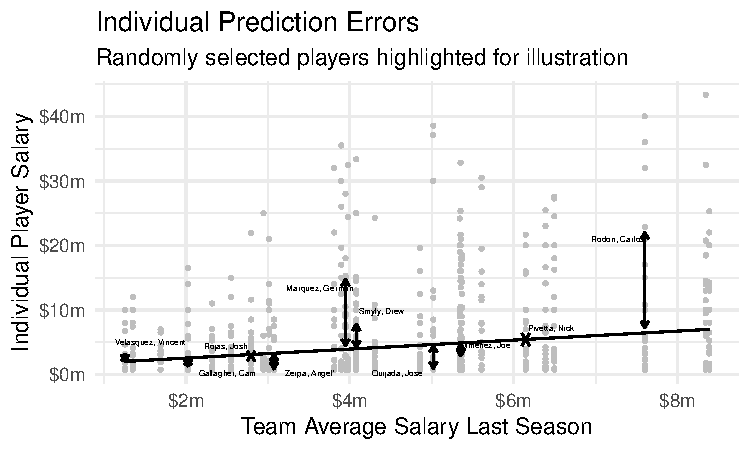
\includegraphics[width = \textwidth]{figures/individual_prediction_errors}
\end{frame}

\begin{frame}
$$
R^2 = 1 - \frac{\overbrace{\V\left(Y - \hat{Y}\right)}^\text{Variance of Errors}}{\underbrace{\V(Y)}_\text{Variance of Y}}
$$
Limiting cases:
\begin{itemize}
\item 1 = perfect prediction
\item 0 = predicted same value for all cases
\end{itemize}
This example: $R^2 = 0.058$
\end{frame}

\begin{frame}
What if the goal is to estimate for subgroups\\instead of to predict for individuals?
\end{frame}

\begin{frame}
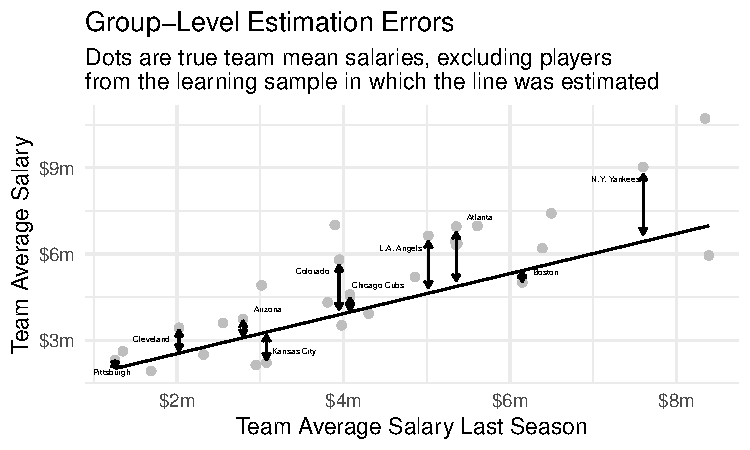
\includegraphics[width = \textwidth]{figures/team_prediction_errors}
\end{frame}

\begin{frame}
$$
R^2_\text{Group} = 1 - \frac{\text{V}\left(\hat{Y}_\text{Team} - \bar{Y}_\text{Team}\right)}{\text{V}(\bar{Y}_\text{Team})}
$$
Variance of team-level prediction errors\\over variance of team-level means\footnote{$R^2_\text{Group}$ is not widely used, but I think it is useful here.\\{}} \vskip .2in
In this example: $R^2_\text{Group} = 0.672$
\end{frame}

\begin{frame}{Individual prediction and subgroup estimation:\\Two very different goals?}

\begin{tikzpicture}[x = \textwidth, y = .8\textheight]
\node at (0,0) {};
\node at (1,1) {};
\node[anchor = north west] at (0,1) {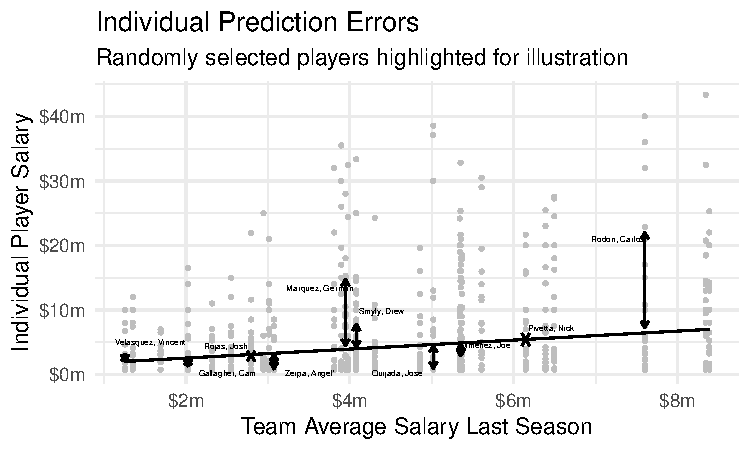
\includegraphics[width = .5\textwidth]{figures/individual_prediction_errors}};
\node[anchor = north west] at (.5,1) {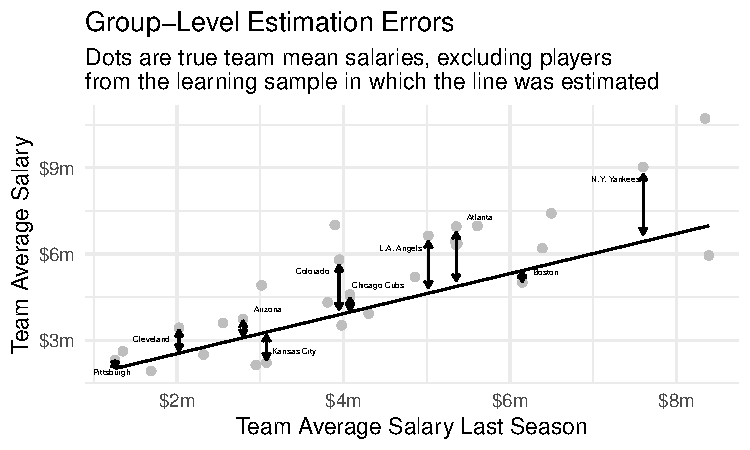
\includegraphics[width = .5\textwidth]{figures/team_prediction_errors}};
\node[anchor = north] at (.25,.5) {$R^2 = 0.058$};
\node[anchor = north] at (.75,.5) {$R^2_\text{Group} = 0.672$};
\end{tikzpicture}

\end{frame}

\begin{frame}{Expected squared prediction error}{Individual-level errors}
$$
\underbrace{\text{ESPE}(\hat{f})}_{\substack{\text{Expected Squared}\\\text{Prediction Error}}} = \text{E}\left[\left(Y - \hat{f}(\vec{X})\right)^2\right]
$$ \vskip .2in
\bgray{In words:}\\
The squared prediction error that occurs on average for a unit sampled at random from the population
\end{frame}

\begin{frame}{Expected squared estimation error}{Errors for estimating subgroup means}
$$
\underbrace{\text{ESEE}(\hat{f})}_{\substack{\text{Expected Squared}\\\text{Estimation Error}}} = \text{E}\left[\left(\text{E}(Y\mid\vec{X}) - \hat{f}(\vec{X})\right)^2\right]
$$ \vskip .2in
\bgray{In words:}\\
The squared error when estimating conditional means given $\vec{X}$,\\
averaged over the distribution of the predictors $\vec{X}$
\end{frame}

\begin{frame}{Within-group variance}{Spread of individual outcomes within groups}
$$
\text{E}\left[\V\left(Y\mid\vec{X})\right)\right]
$$ \vskip .2in
\bgray{In words:}\\
Within each subgroup defined by $\vec{X}$, outcomes vary.\\
This is the average value of the within-group variance,\\
with the average taken over $\vec{X}$
\end{frame}

\begin{frame}[t]{Decomposition of individual prediction error}
$$
\underbrace{\text{ESPE}(\hat{f})}_{\substack{\text{Expected Squared}\\\text{Prediction Error}}}  = \underbrace{\text{ESEE}(\hat{f})}_{\substack{\text{Expected Squared}\\\text{Estimation Error}}} + \underbrace{\text{E}\left[\text{V}(Y\mid\vec{X})\right]}_{\substack{\text{Expected Within-}\\\text{Group Variance}}} 
$$ \vskip .2in \pause
\begin{tikzpicture}[x = \textwidth, y = .8\textheight]
\node[anchor = north west] at (0,1) {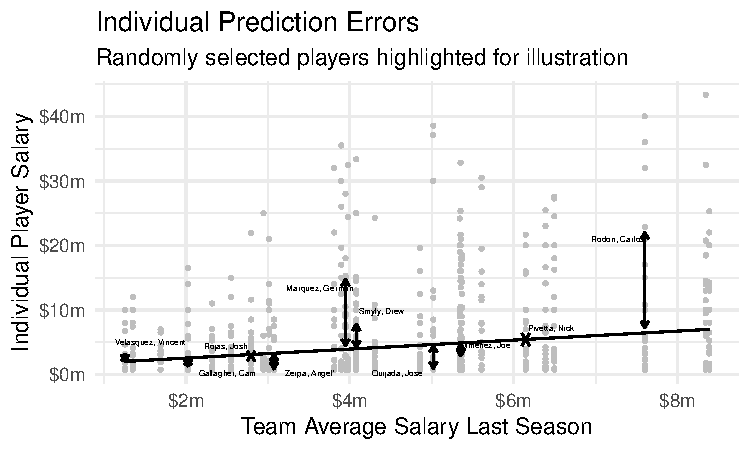
\includegraphics[width = .5\textwidth]{figures/individual_prediction_errors}};
\node[anchor = north west] at (.5,1) {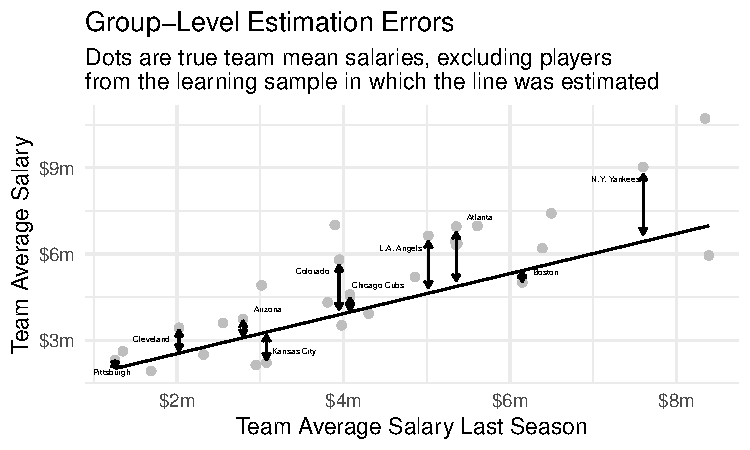
\includegraphics[width = .5\textwidth]{figures/team_prediction_errors}};
\end{tikzpicture}
\end{frame}

\begin{frame}[t]{Decomposition of individual prediction error}
$$
\underbrace{\text{ESPE}(\hat{f})}_{\substack{\text{Expected Squared}\\\text{Prediction Error}}}  = \underbrace{\text{ESEE}(\hat{f})}_{\substack{\text{Expected Squared}\\\text{Estimation Error}}} + \underbrace{\text{E}\left[\text{V}(Y\mid\vec{X})\right]}_{\substack{\text{Expected Within-}\\\text{Group Variance}}} 
$$ \vskip .2in 
Suppose $\hat{f}_1$ and $\hat{f}_2$ are prediction functions \\ \pause
Suppose $\text{ESPE}(\hat{f}_1)<\text{ESPE}(\hat{f}_2)$ \\ \pause
Then
$$\text{ESEE}(\hat{f}_1)\quad\only<3>{?}\only<4->{<}\quad\text{ESEE}(\hat{f}_2)$$ \pause\pause
Strategy: \pause
\begin{itemize}
\item With many candidate algorithms $\hat{f}_1,\hat{f}_2,\dots$ \pause
\item choose the one that minimizes ESPE (individual prediction)\pause
\item It will also minimize ESEE \qquad\qquad\quad (group estimation)
\end{itemize}
\end{frame}

\section{Why Out-of-Sample Prediction}

\tcframe

\begin{frame}{k-nearest neighbors}

10 sampled players per team
\begin{itemize}
\item Dodger sample mean might be noisy
\item Could pool with similar teams defined by past mean salary
\begin{itemize}
\item Dodgers: 8.39m
\item 1st-nearest neighbor. NY Mets: 8.34m
\item 2nd-nearest neighbor. NY Yankees: 7.60m
\item 3rd-nearest neighbor. Philadelphia: 6.50m
\end{itemize}
\item How does performance change with the number of neighbors included?
\begin{itemize}
\item measured by mean squared prediction error
\end{itemize}
\end{itemize}

\end{frame}

\begin{frame}
\includegraphics<1>[width = \textwidth]{figures/knn_0}
\includegraphics<2>[width = \textwidth]{figures/knn_1}
\includegraphics<3>[width = \textwidth]{figures/knn_2}
\includegraphics<4>[width = \textwidth]{figures/knn_3}
\includegraphics<5>[width = \textwidth]{figures/knn_4}
\includegraphics<6>[width = \textwidth]{figures/knn_5}
\includegraphics<7>[width = \textwidth]{figures/knn_10}
\includegraphics<8>[width = \textwidth]{figures/knn_15}
\includegraphics<9>[width = \textwidth]{figures/knn_20}
\includegraphics<10>[width = \textwidth]{figures/knn_25}
\end{frame}

\begin{frame}
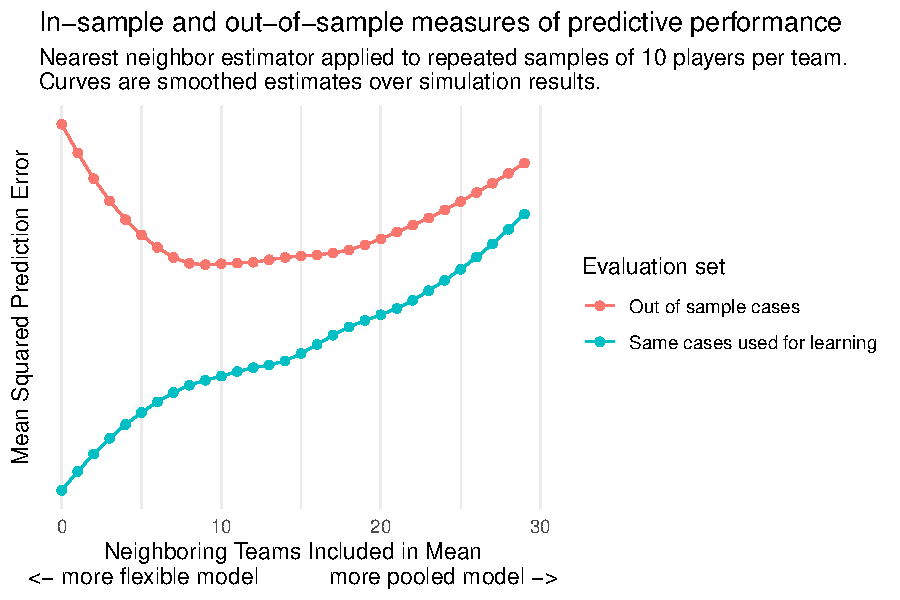
\includegraphics[width = \textwidth]{figures/knn_29}
\end{frame}

\section{Sample Splitting}

\tcframe

\begin{frame}
You have one sample.\\
How do you estimate out-of-sample performance?
\end{frame}

\begin{frame}
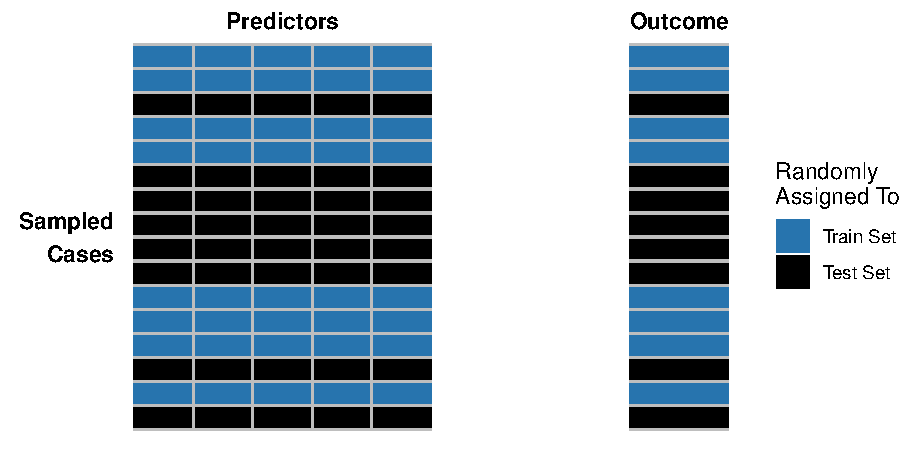
\includegraphics[width = \textwidth]{figures/randomize_split}
\end{frame}

\begin{frame}
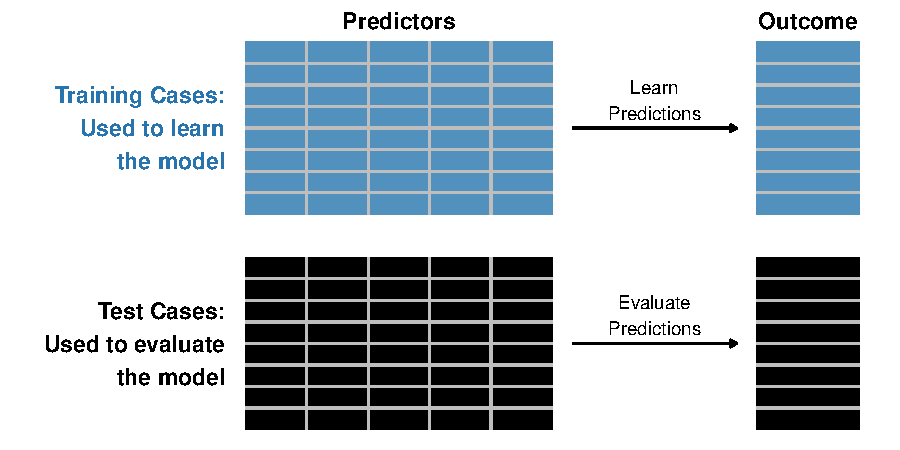
\includegraphics[width = \textwidth]{figures/train_test}
\end{frame}

\begin{frame}{Exercise: Conduct a sample split in code}

\begin{enumerate}
\item Sample 10 players per team
\item Take a 50-50 sample split stratified by team
\item Fit a linear regression in the train set
\item Predict in the test set
\item Report mean squared error
\end{enumerate}

\end{frame}

\begin{frame}{Sample splitting for parameter tuning: Ridge regression}
$$
\E(\text{Player Salary}\mid\text{Team} = t) = \alpha + \beta_t
$$
$$
\left\{\hat\alpha,\hat{\vec\beta}\right\} = \underset{\tilde\alpha,\tilde{\vec\beta}}{\text{arg min}} \underbrace{\sum_{i=1}^n\left(Y_i - \left(\tilde\alpha + \tilde\beta_{t(i)}\right)\right)}_\text{Prediction Error} + \underbrace{\lambda \sum_t \tilde\beta_t^2}_\text{Penalty}
$$
How do we choose $\lambda$?
\end{frame}

\begin{frame}
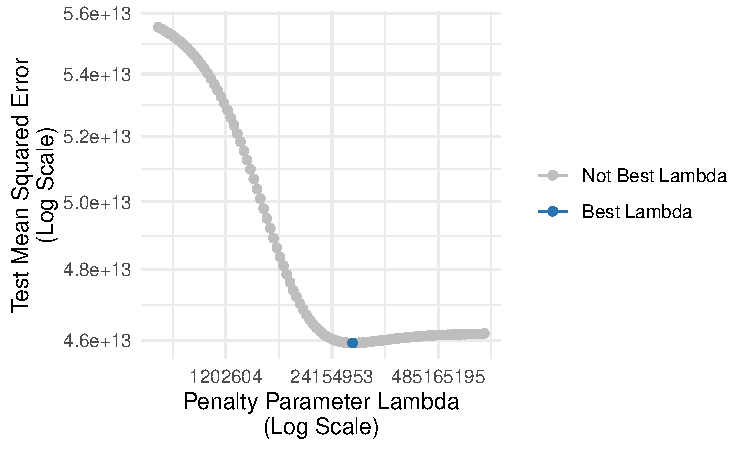
\includegraphics[width = \textwidth]{figures/choosing_lambda}
\end{frame}

\section{Cross Validation}

\tcframe

\begin{frame}{Cross Validation}

A train test split loses lots of data to testing. \vskip .2in
Is there a way to bring it back?

\end{frame}

\begin{frame}{Cross Validation}
\begin{tikzpicture}[x = \textwidth, y = .8\textheight]
\node at (0,0) {};
\node at (1,1) {};
\node[anchor = north west, align = center] at (0,1) {Randomize\\to 5 folds};
\node[anchor = north west] at (0,.9) {
\includegraphics[scale = .8]{figures/five_folds}};
\node<2->[anchor = north, align = center] at (.55,1) {Iteratively use each as the test set};
\node<3->[anchor = north west] at (.2,.9) {
\includegraphics[scale = .8]{figures/five_folds_1}};
\node<4->[anchor = north west] at (.35,.9) {
\includegraphics[scale = .8]{figures/five_folds_2}};
\node<5->[anchor = north west] at (.5,.9) {
\includegraphics[scale = .8]{figures/five_folds_3}};
\node<6->[anchor = north west] at (.65,.9) {
\includegraphics[scale = .8]{figures/five_folds_4}};
\node<7->[anchor = north west] at (.8,.9) {
\includegraphics[scale = .8]{figures/five_folds_5}};
\node<8->[anchor = north, align = center] at (.55,.1) {Average prediction error over folds};
\end{tikzpicture}
\end{frame}

\begin{frame}
Out-of-sample predictive performance is not just for tuning parameters. \vskip .2in
It can help you choose your algorithm.
\end{frame}

\begin{frame}
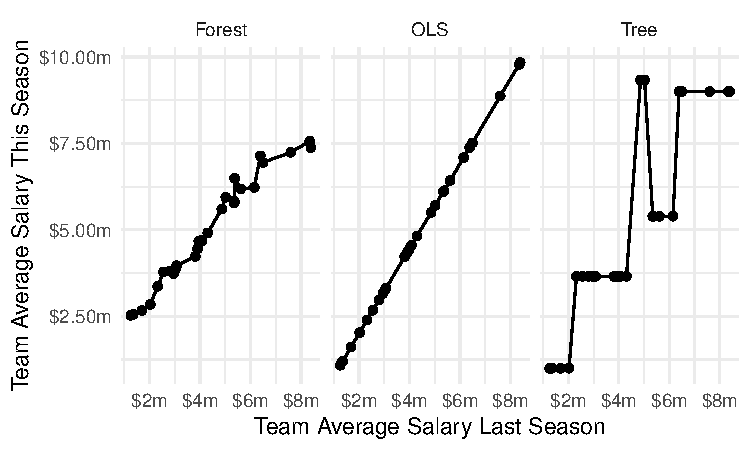
\includegraphics[width = \textwidth]{figures/many_algorithm_predictions}
\end{frame}

\begin{frame}
\includegraphics[width = \textwidth]{figures/many_algorithm_mse}
\end{frame}

\section{Writing Task}

\tcframe

\begin{frame}{Writing Task: A possible abstract}
Imagine that your results came out really amazing.\\
Write the abstract of your paper with these imaginary results.\vskip .2in
\begin{itemize}
\item Minimize jargon. Write for a New York Times reader.
\item Emphasize big claims, not buried in statistics
\end{itemize} \vskip .2in
Goal is to ask a high-impact question.\\If possible, also write the abstract if results were opposite. \vskip .2in
If your abstract is not compelling,\\you might consider finding a new research question.

\end{frame}





\goalsframe

\end{document}